% Numeros de ligne retires pour accelerer la compilation (Overleaf gratuit).
% Pour les remettre : \documentclass[twocolumn,lineno]{ICCKjournal}
\documentclass[twocolumn]{ICCKjournal}

% --- Packages essentiels ---
\usepackage[T1]{fontenc}
\usepackage[french]{babel}
\usepackage{amsmath, amssymb, graphicx, booktabs, hyperref, subcaption}
\usepackage{xcolor}

% --- Résultats chiffrés : générés par le notebook (cellule 15) ---
% Tant que le notebook n'a pas tourné, chaque valeur s'affiche « ? » en rouge.
\newcommand{\tbd}{\textcolor{red}{\textbf{?}}}
% Genere automatiquement par le notebook ArchiGAN-SL (cellule 15).
% device=Tesla T4 quick=False
\newcommand{\resAblLambdaCinqPZeroDiversite}{34{,}2\,\%}
\newcommand{\resAblLambdaCinqPZeroPlausibiliteSnap}{95{,}1\,\%}
\newcommand{\resAblLambdaCinqPZeroRespectBrut}{99{,}4\,\%}
\newcommand{\resAblLambdaCinqZeroPZeroDiversite}{34{,}1\,\%}
\newcommand{\resAblLambdaCinqZeroPZeroPlausibiliteSnap}{94{,}3\,\%}
\newcommand{\resAblLambdaCinqZeroPZeroRespectBrut}{100{,}0\,\%}
\newcommand{\resAblLambdaUnCinqPZeroDiversite}{36{,}6\,\%}
\newcommand{\resAblLambdaUnCinqPZeroPlausibiliteSnap}{94{,}8\,\%}
\newcommand{\resAblLambdaUnCinqPZeroRespectBrut}{99{,}8\,\%}
\newcommand{\resAblLambdaUnPZeroDiversite}{35{,}3\,\%}
\newcommand{\resAblLambdaUnPZeroPlausibiliteSnap}{90{,}8\,\%}
\newcommand{\resAblLambdaUnPZeroRespectBrut}{97{,}0\,\%}
\newcommand{\resAblLambdaZeroPZeroDiversite}{38{,}8\,\%}
\newcommand{\resAblLambdaZeroPZeroPlausibiliteSnap}{92{,}4\,\%}
\newcommand{\resAblLambdaZeroPZeroRespectBrut}{94{,}7\,\%}
\newcommand{\resDsAcceptance}{98{,}0\,\%}
\newcommand{\resDsMeanRooms}{8{,}28}
\newcommand{\resDsN}{20\,000}
\newcommand{\resDsUnique}{984}
\newcommand{\resDsUniquePieces}{104}
\newcommand{\resLeakSlBaselineExact}{3{,}1\,\%}
\newcommand{\resLeakSlBaselineParEntree}{69{,}5\,\%}
\newcommand{\resLeakSlExact}{46{,}7\,\%}
\newcommand{\resLeakSlParEntree}{94{,}9\,\%}
\newcommand{\resLeakSplitfedBaselineExact}{3{,}1\,\%}
\newcommand{\resLeakSplitfedBaselineParEntree}{69{,}5\,\%}
\newcommand{\resLeakSplitfedBruitBaselineExact}{3{,}1\,\%}
\newcommand{\resLeakSplitfedBruitBaselineParEntree}{69{,}5\,\%}
\newcommand{\resLeakSplitfedBruitExact}{0{,}4\,\%}
\newcommand{\resLeakSplitfedBruitParEntree}{68{,}0\,\%}
\newcommand{\resLeakSplitfedExact}{52{,}9\,\%}
\newcommand{\resLeakSplitfedParEntree}{95{,}0\,\%}
\newcommand{\resParamsD}{30\,721}
\newcommand{\resParamsG}{34\,319}
\newcommand{\resPlanAleatoireAccesDirect}{99{,}9\,\%}
\newcommand{\resPlanAleatoireAccesDirectCi}{0{,}1}
\newcommand{\resPlanAleatoireAdjacence}{93{,}6\,\%}
\newcommand{\resPlanAleatoireAdjacenceCi}{0{,}8}
\newcommand{\resPlanAleatoireCompacite}{73{,}7\,\%}
\newcommand{\resPlanAleatoireCompaciteCi}{0{,}3}
\newcommand{\resPlanAleatoireConnectivite}{100{,}0\,\%}
\newcommand{\resPlanAleatoireConnectiviteCi}{0{,}0}
\newcommand{\resPlanAleatoireConnexe}{100{,}0\,\%}
\newcommand{\resPlanAleatoireConnexeCi}{0{,}0}
\newcommand{\resPlanAleatoireDiversite}{89{,}5\,\%}
\newcommand{\resPlanAleatoireDiversiteCi}{0{,}7}
\newcommand{\resPlanAleatoireDiversiteGraphe}{45{,}9\,\%}
\newcommand{\resPlanAleatoireDiversiteGrapheCi}{1{,}0}
\newcommand{\resPlanAleatoireEcartSurface}{5{,}6\,\%}
\newcommand{\resPlanAleatoireEcartSurfaceCi}{0{,}0}
\newcommand{\resPlanAleatoireEntree}{99{,}7\,\%}
\newcommand{\resPlanAleatoireEntreeCi}{0{,}3}
\newcommand{\resPlanAleatoirePlacement}{100{,}0\,\%}
\newcommand{\resPlanAleatoirePlacementCi}{0{,}0}
\newcommand{\resPlanAleatoirePlausibilite}{17{,}0\,\%}
\newcommand{\resPlanAleatoirePlausibiliteCi}{2{,}2}
\newcommand{\resPlanAleatoirePortesLegales}{98{,}5\,\%}
\newcommand{\resPlanAleatoirePortesLegalesCi}{0{,}3}
\newcommand{\resPlanAleatoirePortesPiecePrivee}{1{,}22}
\newcommand{\resPlanAleatoireRespectBrut}{100{,}0\,\%}
\newcommand{\resPlanAleatoireRespectBrutCi}{0{,}0}
\newcommand{\resPlanAleatoireRespectGraphe}{95{,}4\,\%}
\newcommand{\resPlanAleatoireRespectGrapheCi}{2{,}6}
\newcommand{\resPlanAleatoireRespectPlan}{99{,}8\,\%}
\newcommand{\resPlanAleatoireRespectPlanCi}{0{,}1}
\newcommand{\resPlanAleatoireSansPorteInterdite}{100{,}0\,\%}
\newcommand{\resPlanAleatoireSansPorteInterditeCi}{0{,}0}
\newcommand{\resPlanAleatoireTCgan}{0{,}0}
\newcommand{\resPlanAleatoireTLayout}{2{,}8}
\newcommand{\resPlanAleatoireTTotal}{3{,}0}
\newcommand{\resPlanCganBrutAccesDirect}{100{,}0\,\%}
\newcommand{\resPlanCganBrutAccesDirectCi}{0{,}0}
\newcommand{\resPlanCganBrutAdjacence}{89{,}0\,\%}
\newcommand{\resPlanCganBrutAdjacenceCi}{1{,}0}
\newcommand{\resPlanCganBrutCompacite}{73{,}6\,\%}
\newcommand{\resPlanCganBrutCompaciteCi}{0{,}3}
\newcommand{\resPlanCganBrutConnectivite}{100{,}0\,\%}
\newcommand{\resPlanCganBrutConnectiviteCi}{0{,}0}
\newcommand{\resPlanCganBrutConnexe}{100{,}0\,\%}
\newcommand{\resPlanCganBrutConnexeCi}{0{,}0}
\newcommand{\resPlanCganBrutDiversite}{52{,}3\,\%}
\newcommand{\resPlanCganBrutDiversiteCi}{1{,}0}
\newcommand{\resPlanCganBrutDiversiteGraphe}{31{,}3\,\%}
\newcommand{\resPlanCganBrutDiversiteGrapheCi}{0{,}8}
\newcommand{\resPlanCganBrutEcartSurface}{5{,}0\,\%}
\newcommand{\resPlanCganBrutEcartSurfaceCi}{0{,}0}
\newcommand{\resPlanCganBrutEntree}{100{,}0\,\%}
\newcommand{\resPlanCganBrutEntreeCi}{0{,}0}
\newcommand{\resPlanCganBrutPlacement}{100{,}0\,\%}
\newcommand{\resPlanCganBrutPlacementCi}{0{,}0}
\newcommand{\resPlanCganBrutPlausibilite}{84{,}7\,\%}
\newcommand{\resPlanCganBrutPlausibiliteCi}{2{,}1}
\newcommand{\resPlanCganBrutPortesLegales}{99{,}1\,\%}
\newcommand{\resPlanCganBrutPortesLegalesCi}{0{,}2}
\newcommand{\resPlanCganBrutPortesPiecePrivee}{1{,}23}
\newcommand{\resPlanCganBrutRespectBrut}{98{,}4\,\%}
\newcommand{\resPlanCganBrutRespectBrutCi}{0{,}4}
\newcommand{\resPlanCganBrutRespectGraphe}{99{,}4\,\%}
\newcommand{\resPlanCganBrutRespectGrapheCi}{0{,}9}
\newcommand{\resPlanCganBrutRespectPlan}{98{,}4\,\%}
\newcommand{\resPlanCganBrutRespectPlanCi}{0{,}4}
\newcommand{\resPlanCganBrutSansPorteInterdite}{100{,}0\,\%}
\newcommand{\resPlanCganBrutSansPorteInterditeCi}{0{,}0}
\newcommand{\resPlanCganBrutTCgan}{0{,}0}
\newcommand{\resPlanCganBrutTLayout}{3{,}1}
\newcommand{\resPlanCganBrutTTotal}{3{,}3}
\newcommand{\resPlanCganSnapAccesDirect}{100{,}0\,\%}
\newcommand{\resPlanCganSnapAccesDirectCi}{0{,}0}
\newcommand{\resPlanCganSnapAdjacence}{89{,}1\,\%}
\newcommand{\resPlanCganSnapAdjacenceCi}{1{,}0}
\newcommand{\resPlanCganSnapCompacite}{73{,}9\,\%}
\newcommand{\resPlanCganSnapCompaciteCi}{0{,}3}
\newcommand{\resPlanCganSnapConnectivite}{100{,}0\,\%}
\newcommand{\resPlanCganSnapConnectiviteCi}{0{,}0}
\newcommand{\resPlanCganSnapConnexe}{100{,}0\,\%}
\newcommand{\resPlanCganSnapConnexeCi}{0{,}0}
\newcommand{\resPlanCganSnapDiversite}{51{,}9\,\%}
\newcommand{\resPlanCganSnapDiversiteCi}{1{,}0}
\newcommand{\resPlanCganSnapDiversiteGraphe}{32{,}1\,\%}
\newcommand{\resPlanCganSnapDiversiteGrapheCi}{0{,}9}
\newcommand{\resPlanCganSnapEcartSurface}{4{,}6\,\%}
\newcommand{\resPlanCganSnapEcartSurfaceCi}{0{,}0}
\newcommand{\resPlanCganSnapEntree}{99{,}9\,\%}
\newcommand{\resPlanCganSnapEntreeCi}{0{,}2}
\newcommand{\resPlanCganSnapGrapheReglesAccesDirect}{100{,}0\,\%}
\newcommand{\resPlanCganSnapGrapheReglesAccesDirectCi}{0{,}0}
\newcommand{\resPlanCganSnapGrapheReglesAdjacence}{92{,}1\,\%}
\newcommand{\resPlanCganSnapGrapheReglesAdjacenceCi}{0{,}7}
\newcommand{\resPlanCganSnapGrapheReglesCompacite}{73{,}7\,\%}
\newcommand{\resPlanCganSnapGrapheReglesCompaciteCi}{0{,}3}
\newcommand{\resPlanCganSnapGrapheReglesConnectivite}{100{,}0\,\%}
\newcommand{\resPlanCganSnapGrapheReglesConnectiviteCi}{0{,}0}
\newcommand{\resPlanCganSnapGrapheReglesConnexe}{100{,}0\,\%}
\newcommand{\resPlanCganSnapGrapheReglesConnexeCi}{0{,}0}
\newcommand{\resPlanCganSnapGrapheReglesDiversite}{22{,}0\,\%}
\newcommand{\resPlanCganSnapGrapheReglesDiversiteCi}{0{,}5}
\newcommand{\resPlanCganSnapGrapheReglesDiversiteGraphe}{14{,}0\,\%}
\newcommand{\resPlanCganSnapGrapheReglesDiversiteGrapheCi}{0{,}4}
\newcommand{\resPlanCganSnapGrapheReglesEcartSurface}{4{,}8\,\%}
\newcommand{\resPlanCganSnapGrapheReglesEcartSurfaceCi}{0{,}0}
\newcommand{\resPlanCganSnapGrapheReglesEntree}{99{,}8\,\%}
\newcommand{\resPlanCganSnapGrapheReglesEntreeCi}{0{,}3}
\newcommand{\resPlanCganSnapGrapheReglesPlacement}{100{,}0\,\%}
\newcommand{\resPlanCganSnapGrapheReglesPlacementCi}{0{,}0}
\newcommand{\resPlanCganSnapGrapheReglesPlausibilite}{82{,}4\,\%}
\newcommand{\resPlanCganSnapGrapheReglesPlausibiliteCi}{2{,}3}
\newcommand{\resPlanCganSnapGrapheReglesPortesLegales}{99{,}2\,\%}
\newcommand{\resPlanCganSnapGrapheReglesPortesLegalesCi}{0{,}2}
\newcommand{\resPlanCganSnapGrapheReglesPortesPiecePrivee}{1{,}25}
\newcommand{\resPlanCganSnapGrapheReglesRespectBrut}{98{,}4\,\%}
\newcommand{\resPlanCganSnapGrapheReglesRespectBrutCi}{0{,}4}
\newcommand{\resPlanCganSnapGrapheReglesRespectGraphe}{50{,}8\,\%}
\newcommand{\resPlanCganSnapGrapheReglesRespectGrapheCi}{5{,}6}
\newcommand{\resPlanCganSnapGrapheReglesRespectPlan}{97{,}6\,\%}
\newcommand{\resPlanCganSnapGrapheReglesRespectPlanCi}{0{,}4}
\newcommand{\resPlanCganSnapGrapheReglesSansPorteInterdite}{100{,}0\,\%}
\newcommand{\resPlanCganSnapGrapheReglesSansPorteInterditeCi}{0{,}0}
\newcommand{\resPlanCganSnapGrapheReglesTCgan}{0{,}0}
\newcommand{\resPlanCganSnapGrapheReglesTLayout}{2{,}3}
\newcommand{\resPlanCganSnapGrapheReglesTTotal}{2{,}5}
\newcommand{\resPlanCganSnapPlacement}{100{,}0\,\%}
\newcommand{\resPlanCganSnapPlacementCi}{0{,}0}
\newcommand{\resPlanCganSnapPlacementVDeuxAccesDirect}{98{,}6\,\%}
\newcommand{\resPlanCganSnapPlacementVDeuxAccesDirectCi}{0{,}2}
\newcommand{\resPlanCganSnapPlacementVDeuxAdjacence}{89{,}4\,\%}
\newcommand{\resPlanCganSnapPlacementVDeuxAdjacenceCi}{0{,}8}
\newcommand{\resPlanCganSnapPlacementVDeuxCompacite}{63{,}7\,\%}
\newcommand{\resPlanCganSnapPlacementVDeuxCompaciteCi}{0{,}5}
\newcommand{\resPlanCganSnapPlacementVDeuxConnectivite}{100{,}0\,\%}
\newcommand{\resPlanCganSnapPlacementVDeuxConnectiviteCi}{0{,}0}
\newcommand{\resPlanCganSnapPlacementVDeuxConnexe}{100{,}0\,\%}
\newcommand{\resPlanCganSnapPlacementVDeuxConnexeCi}{0{,}0}
\newcommand{\resPlanCganSnapPlacementVDeuxDiversite}{51{,}9\,\%}
\newcommand{\resPlanCganSnapPlacementVDeuxDiversiteCi}{1{,}0}
\newcommand{\resPlanCganSnapPlacementVDeuxDiversiteGraphe}{39{,}5\,\%}
\newcommand{\resPlanCganSnapPlacementVDeuxDiversiteGrapheCi}{1{,}0}
\newcommand{\resPlanCganSnapPlacementVDeuxEcartSurface}{20{,}5\,\%}
\newcommand{\resPlanCganSnapPlacementVDeuxEcartSurfaceCi}{0{,}0}
\newcommand{\resPlanCganSnapPlacementVDeuxEntree}{0{,}0\,\%}
\newcommand{\resPlanCganSnapPlacementVDeuxEntreeCi}{0{,}0}
\newcommand{\resPlanCganSnapPlacementVDeuxPlacement}{100{,}0\,\%}
\newcommand{\resPlanCganSnapPlacementVDeuxPlacementCi}{0{,}0}
\newcommand{\resPlanCganSnapPlacementVDeuxPlausibilite}{80{,}5\,\%}
\newcommand{\resPlanCganSnapPlacementVDeuxPlausibiliteCi}{2{,}3}
\newcommand{\resPlanCganSnapPlacementVDeuxPortesLegales}{98{,}7\,\%}
\newcommand{\resPlanCganSnapPlacementVDeuxPortesLegalesCi}{0{,}2}
\newcommand{\resPlanCganSnapPlacementVDeuxPortesPiecePrivee}{1{,}70}
\newcommand{\resPlanCganSnapPlacementVDeuxRespectBrut}{98{,}4\,\%}
\newcommand{\resPlanCganSnapPlacementVDeuxRespectBrutCi}{0{,}4}
\newcommand{\resPlanCganSnapPlacementVDeuxRespectGraphe}{52{,}0\,\%}
\newcommand{\resPlanCganSnapPlacementVDeuxRespectGrapheCi}{6{,}0}
\newcommand{\resPlanCganSnapPlacementVDeuxRespectPlan}{97{,}8\,\%}
\newcommand{\resPlanCganSnapPlacementVDeuxRespectPlanCi}{0{,}4}
\newcommand{\resPlanCganSnapPlacementVDeuxSansPorteInterdite}{96{,}5\,\%}
\newcommand{\resPlanCganSnapPlacementVDeuxSansPorteInterditeCi}{1{,}1}
\newcommand{\resPlanCganSnapPlacementVDeuxTCgan}{0{,}0}
\newcommand{\resPlanCganSnapPlacementVDeuxTLayout}{38{,}3}
\newcommand{\resPlanCganSnapPlacementVDeuxTTotal}{38{,}5}
\newcommand{\resPlanCganSnapPlausibilite}{80{,}5\,\%}
\newcommand{\resPlanCganSnapPlausibiliteCi}{2{,}3}
\newcommand{\resPlanCganSnapPortesLegales}{99{,}1\,\%}
\newcommand{\resPlanCganSnapPortesLegalesCi}{0{,}2}
\newcommand{\resPlanCganSnapPortesPiecePrivee}{1{,}22}
\newcommand{\resPlanCganSnapRespectBrut}{98{,}4\,\%}
\newcommand{\resPlanCganSnapRespectBrutCi}{0{,}4}
\newcommand{\resPlanCganSnapRespectGraphe}{99{,}4\,\%}
\newcommand{\resPlanCganSnapRespectGrapheCi}{0{,}9}
\newcommand{\resPlanCganSnapRespectPlan}{100{,}0\,\%}
\newcommand{\resPlanCganSnapRespectPlanCi}{0{,}0}
\newcommand{\resPlanCganSnapSansPorteInterdite}{100{,}0\,\%}
\newcommand{\resPlanCganSnapSansPorteInterditeCi}{0{,}0}
\newcommand{\resPlanCganSnapTCgan}{0{,}0}
\newcommand{\resPlanCganSnapTLayout}{2{,}2}
\newcommand{\resPlanCganSnapTRender}{212{,}8}
\newcommand{\resPlanCganSnapTTotal}{2{,}4}
\newcommand{\resPlanCganSnapUnEssaiAccesDirect}{99{,}3\,\%}
\newcommand{\resPlanCganSnapUnEssaiAccesDirectCi}{0{,}2}
\newcommand{\resPlanCganSnapUnEssaiAdjacence}{89{,}4\,\%}
\newcommand{\resPlanCganSnapUnEssaiAdjacenceCi}{1{,}0}
\newcommand{\resPlanCganSnapUnEssaiCompacite}{73{,}6\,\%}
\newcommand{\resPlanCganSnapUnEssaiCompaciteCi}{0{,}3}
\newcommand{\resPlanCganSnapUnEssaiConnectivite}{100{,}0\,\%}
\newcommand{\resPlanCganSnapUnEssaiConnectiviteCi}{0{,}0}
\newcommand{\resPlanCganSnapUnEssaiConnexe}{100{,}0\,\%}
\newcommand{\resPlanCganSnapUnEssaiConnexeCi}{0{,}0}
\newcommand{\resPlanCganSnapUnEssaiDiversite}{51{,}9\,\%}
\newcommand{\resPlanCganSnapUnEssaiDiversiteCi}{1{,}0}
\newcommand{\resPlanCganSnapUnEssaiDiversiteGraphe}{32{,}5\,\%}
\newcommand{\resPlanCganSnapUnEssaiDiversiteGrapheCi}{0{,}9}
\newcommand{\resPlanCganSnapUnEssaiEcartSurface}{4{,}7\,\%}
\newcommand{\resPlanCganSnapUnEssaiEcartSurfaceCi}{0{,}0}
\newcommand{\resPlanCganSnapUnEssaiEntree}{99{,}9\,\%}
\newcommand{\resPlanCganSnapUnEssaiEntreeCi}{0{,}2}
\newcommand{\resPlanCganSnapUnEssaiPlacement}{100{,}0\,\%}
\newcommand{\resPlanCganSnapUnEssaiPlacementCi}{0{,}0}
\newcommand{\resPlanCganSnapUnEssaiPlausibilite}{80{,}5\,\%}
\newcommand{\resPlanCganSnapUnEssaiPlausibiliteCi}{2{,}3}
\newcommand{\resPlanCganSnapUnEssaiPortesLegales}{99{,}1\,\%}
\newcommand{\resPlanCganSnapUnEssaiPortesLegalesCi}{0{,}2}
\newcommand{\resPlanCganSnapUnEssaiPortesPiecePrivee}{1{,}24}
\newcommand{\resPlanCganSnapUnEssaiRespectBrut}{98{,}4\,\%}
\newcommand{\resPlanCganSnapUnEssaiRespectBrutCi}{0{,}4}
\newcommand{\resPlanCganSnapUnEssaiRespectGraphe}{99{,}2\,\%}
\newcommand{\resPlanCganSnapUnEssaiRespectGrapheCi}{1{,}0}
\newcommand{\resPlanCganSnapUnEssaiRespectPlan}{100{,}0\,\%}
\newcommand{\resPlanCganSnapUnEssaiRespectPlanCi}{0{,}1}
\newcommand{\resPlanCganSnapUnEssaiSansPorteInterdite}{100{,}0\,\%}
\newcommand{\resPlanCganSnapUnEssaiSansPorteInterditeCi}{0{,}0}
\newcommand{\resPlanCganSnapUnEssaiTCgan}{0{,}0}
\newcommand{\resPlanCganSnapUnEssaiTLayout}{1{,}8}
\newcommand{\resPlanCganSnapUnEssaiTTotal}{2{,}0}
\newcommand{\resPlanPriorAccesDirect}{100{,}0\,\%}
\newcommand{\resPlanPriorAccesDirectCi}{0{,}0}
\newcommand{\resPlanPriorAdjacence}{89{,}4\,\%}
\newcommand{\resPlanPriorAdjacenceCi}{0{,}9}
\newcommand{\resPlanPriorCompacite}{74{,}2\,\%}
\newcommand{\resPlanPriorCompaciteCi}{0{,}3}
\newcommand{\resPlanPriorConnectivite}{100{,}0\,\%}
\newcommand{\resPlanPriorConnectiviteCi}{0{,}0}
\newcommand{\resPlanPriorConnexe}{100{,}0\,\%}
\newcommand{\resPlanPriorConnexeCi}{0{,}0}
\newcommand{\resPlanPriorDiversite}{47{,}2\,\%}
\newcommand{\resPlanPriorDiversiteCi}{1{,}3}
\newcommand{\resPlanPriorDiversiteGraphe}{29{,}3\,\%}
\newcommand{\resPlanPriorDiversiteGrapheCi}{0{,}8}
\newcommand{\resPlanPriorEcartSurface}{5{,}2\,\%}
\newcommand{\resPlanPriorEcartSurfaceCi}{0{,}0}
\newcommand{\resPlanPriorEntree}{99{,}9\,\%}
\newcommand{\resPlanPriorEntreeCi}{0{,}2}
\newcommand{\resPlanPriorPlacement}{100{,}0\,\%}
\newcommand{\resPlanPriorPlacementCi}{0{,}0}
\newcommand{\resPlanPriorPlausibilite}{95{,}5\,\%}
\newcommand{\resPlanPriorPlausibiliteCi}{1{,}2}
\newcommand{\resPlanPriorPortesLegales}{100{,}0\,\%}
\newcommand{\resPlanPriorPortesLegalesCi}{0{,}0}
\newcommand{\resPlanPriorPortesPiecePrivee}{1{,}24}
\newcommand{\resPlanPriorRespectBrut}{100{,}0\,\%}
\newcommand{\resPlanPriorRespectBrutCi}{0{,}0}
\newcommand{\resPlanPriorRespectGraphe}{100{,}0\,\%}
\newcommand{\resPlanPriorRespectGrapheCi}{0{,}0}
\newcommand{\resPlanPriorRespectPlan}{100{,}0\,\%}
\newcommand{\resPlanPriorRespectPlanCi}{0{,}0}
\newcommand{\resPlanPriorSansPorteInterdite}{100{,}0\,\%}
\newcommand{\resPlanPriorSansPorteInterditeCi}{0{,}0}
\newcommand{\resPlanPriorTCgan}{0{,}7}
\newcommand{\resPlanPriorTLayout}{1{,}9}
\newcommand{\resPlanPriorTTotal}{2{,}7}
\newcommand{\resPlanTimeMax}{12{,}8}
\newcommand{\resPlanTimeMedian}{2{,}1}
\newcommand{\resPlanTimeMin}{0{,}7}
\newcommand{\resSlCentraliseEtrangerPlausibilite}{95{,}4\,\%}
\newcommand{\resSlCentraliseEtrangerRespectBrut}{100{,}0\,\%}
\newcommand{\resSlCentraliseGlobalPlausibilite}{94{,}5\,\%}
\newcommand{\resSlCentraliseGlobalRespectBrut}{100{,}0\,\%}
\newcommand{\resSlCentraliseProprePlausibilite}{95{,}3\,\%}
\newcommand{\resSlCentralisePropreRespectBrut}{100{,}0\,\%}
\newcommand{\resSlClientShare}{31{,}9\,\%}
\newcommand{\resSlEpochs}{100}
\newcommand{\resSlFlMoEpoch}{1{,}37}
\newcommand{\resSlLocalEtrangerPlausibilite}{94{,}1\,\%}
\newcommand{\resSlLocalEtrangerRespectBrut}{93{,}6\,\%}
\newcommand{\resSlLocalGlobalPlausibilite}{95{,}6\,\%}
\newcommand{\resSlLocalGlobalRespectBrut}{97{,}0\,\%}
\newcommand{\resSlLocalProprePlausibilite}{98{,}8\,\%}
\newcommand{\resSlLocalPropreRespectBrut}{97{,}5\,\%}
\newcommand{\resSlParamsClient}{18\,208}
\newcommand{\resSlParamsServer}{38\,800}
\newcommand{\resSlSlEtrangerPlausibilite}{89{,}9\,\%}
\newcommand{\resSlSlEtrangerRespectBrut}{90{,}2\,\%}
\newcommand{\resSlSlGlobalPlausibilite}{84{,}7\,\%}
\newcommand{\resSlSlGlobalRespectBrut}{93{,}4\,\%}
\newcommand{\resSlSlMinutes}{4{,}4}
\newcommand{\resSlSlMoEpoch}{37{,}36}
\newcommand{\resSlSlOctetsSample}{2100}
\newcommand{\resSlSlProprePlausibilite}{96{,}2\,\%}
\newcommand{\resSlSlPropreRespectBrut}{89{,}3\,\%}
\newcommand{\resSlSplitfedBruitEtrangerPlausibilite}{98{,}8\,\%}
\newcommand{\resSlSplitfedBruitEtrangerRespectBrut}{93{,}1\,\%}
\newcommand{\resSlSplitfedBruitGlobalPlausibilite}{98{,}2\,\%}
\newcommand{\resSlSplitfedBruitGlobalRespectBrut}{95{,}8\,\%}
\newcommand{\resSlSplitfedBruitMinutes}{4{,}4}
\newcommand{\resSlSplitfedBruitMoEpoch}{37{,}36}
\newcommand{\resSlSplitfedBruitOctetsSample}{2100}
\newcommand{\resSlSplitfedBruitProprePlausibilite}{98{,}8\,\%}
\newcommand{\resSlSplitfedBruitPropreRespectBrut}{93{,}1\,\%}
\newcommand{\resSlSplitfedEtrangerPlausibilite}{98{,}8\,\%}
\newcommand{\resSlSplitfedEtrangerRespectBrut}{96{,}4\,\%}
\newcommand{\resSlSplitfedGlobalPlausibilite}{95{,}6\,\%}
\newcommand{\resSlSplitfedGlobalRespectBrut}{97{,}9\,\%}
\newcommand{\resSlSplitfedMinutes}{4{,}3}
\newcommand{\resSlSplitfedMoEpoch}{37{,}36}
\newcommand{\resSlSplitfedOctetsSample}{2100}
\newcommand{\resSlSplitfedProprePlausibilite}{98{,}8\,\%}
\newcommand{\resSlSplitfedPropreRespectBrut}{96{,}5\,\%}
\newcommand{\resSlSyncMoEpoch}{0{,}44}
\newcommand{\resTrainDacc}{55{,}8\,\%}
\newcommand{\resTrainMinutes}{8{,}7}
\newcommand{\resVecAleatoireDiversite}{74{,}2\,\%}
\newcommand{\resVecAleatoirePlausibilite}{42{,}2\,\%}
\newcommand{\resVecAleatoireRespectBrut}{100{,}0\,\%}
\newcommand{\resVecCganBrutPlausibilite}{93{,}6\,\%}
\newcommand{\resVecCganBrutRespectBrut}{100{,}0\,\%}
\newcommand{\resVecCganSnapDiversite}{39{,}0\,\%}
\newcommand{\resVecCganSnapPlausibilite}{93{,}7\,\%}
\newcommand{\resVecCganSnapRespectBrut}{100{,}0\,\%}
\newcommand{\resVecPriorDiversite}{40{,}5\,\%}
\newcommand{\resVecPriorPlausibilite}{99{,}9\,\%}
\newcommand{\resVecPriorRespectBrut}{100{,}0\,\%}

% Figures exportées par le notebook : figures/fig_*.png
\newcommand{\figorplaceholder}[2]{%
  \IfFileExists{#1}{\includegraphics[width=#2]{#1}}%
  {\fbox{\parbox[c][3cm][c]{0.9#2}{\centering\small\textcolor{red}{Figure à exporter :\\\texttt{\detokenize{#1}}}}}}}
% Remarques de rédaction (à supprimer avant soumission)
\newcommand{\todo}[1]{\textcolor{blue}{[\textit{#1}]}}

% --- Configuration Journal ---
\jnlsetup{
  journal={À déterminer},
  title={Génération de plans architecturaux 2D par cGAN piloté par prompt
         et entraîné en Split Learning : vers une CAO générative
         collaborative et confidentielle},
  ctitle={Génération de plans 2D par cGAN piloté par prompt et Split Learning},
  author={K. Tshibangu Ntumba},
  volume={1},
  number={1},
  year={2026},
  doi={00.0000/icck.2026.01}
}

\articletype{Article de recherche}

\author[1][kennytshibangu9@gmail.com]{Kenny Tshibangu Ntumba}
\affil[1]{Université Nouveaux Horizons, Faculté des Sciences Informatiques,
          Ingénierie Logicielle, Lubumbashi, République Démocratique du Congo}

\begin{document}
\maketitle

% ============================================================
% RÉSUMÉ & MOTS-CLÉS
% ============================================================
\abstract{
\textbf{Contexte :} les logiciels de conception assistée par ordinateur
(CAO) aident à dessiner des plans, mais ne savent pas encore proposer
d'esquisse à partir d'une demande formulée en langage courant. Par
ailleurs, entraîner un modèle génératif suppose en général de rassembler
des plans qui, pour les agences d'architecture, constituent des données
propriétaires.
\textbf{Objectif :} concevoir et évaluer un générateur de plans
résidentiels 2D piloté par une requête textuelle, qui puisse être
entraîné par plusieurs agences sans qu'aucune ne transmette ses données.
\textbf{Méthodes :} la requête est convertie en contraintes partielles
portant sur le programme (nombre de pièces de chaque type) et sur la
structure du graphe de bulles (suite parentale, cuisine fermée, etc.).
Un GAN conditionnel (cGAN) complète les éléments laissés libres, pièces
comme topologie, puis les contraintes explicites sont rétablies et un
placement procédural guidé par le graphe construit le plan. Le cGAN est
entraîné de façon centralisée, puis en Split Learning en U entre trois
agences aux données hétérogènes et un serveur, avec ou sans bruit sur
les activations échangées.
\textbf{Résultats :} sur \resDsN{} programmes, la méthode respecte
\resPlanCganSnapRespectPlan{} des contraintes de la requête dans le plan
final, avec \resPlanCganSnapPlausibilite{} de programmes plausibles,
\resPlanCganSnapPortesLegales{} de portes conformes et un temps médian
de \resPlanTimeMedian{}\,ms par plan. La prédiction du graphe de bulles
fait passer le respect des structures demandées de
\resPlanCganSnapGrapheReglesRespectGraphe{} à
\resPlanCganSnapRespectGraphe{}. En SplitFed, le générateur atteint
\resSlSplitfedGlobalRespectBrut{} de respect des contraintes, contre
\resSlCentraliseGlobalRespectBrut{} en centralisé et
\resSlLocalGlobalRespectBrut{} pour une agence travaillant seule.
Cependant, une attaque par inversion retrouve \resLeakSplitfedExact{}
des programmes à partir des activations échangées ; l'ajout d'un bruit
gaussien ramène ce taux à \resLeakSplitfedBruitExact{} au prix d'environ
deux points de respect.
\textbf{Conclusion :} le Split Learning permet à plusieurs agences
d'obtenir ensemble un générateur proche du modèle centralisé et
meilleur que leurs modèles locaux, à condition de protéger
explicitement les activations échangées.
}

\keywords{GAN conditionnel, Split Learning, SplitFed, génération de plans
architecturaux, conception assistée par ordinateur, confidentialité des
données, requête textuelle}


% ============================================================
\section{Introduction}
% ============================================================

La conception assistée par ordinateur (CAO) occupe aujourd'hui une place
centrale en architecture et en ingénierie~\cite{Gire1983}. Les logiciels
les plus répandus, comme AutoCAD, Revit ou ArchiCAD, restent toutefois
avant tout des outils de dessin. L'architecte y trace chaque mur et
explore les variantes les unes après les autres, ce qui rend la phase
d'esquisse longue et coûteuse. Dans ce contexte, les réseaux
antagonistes génératifs (GANs)~\cite{Goodfellow2020} ont montré qu'il
était possible d'apprendre la distribution d'un ensemble de plans et
d'en proposer de nouveaux~\cite{Huang2018,zheng2020apartment,
Chaillou2020ArchiGAN,Nauata2020HouseGAN}.

Deux difficultés freinent cependant leur usage en agence. La première
tient au contrôle de la génération : un architecte souhaite décrire ce
qu'il veut, par exemple « un T3 avec balcon », plutôt que tirer des plans
au hasard. La seconde tient à la nature des données. Les plans d'une
agence font partie de son savoir-faire, et elle n'acceptera pas
facilement de les confier à un tiers pour entraîner un modèle commun.

Le \emph{Split Learning} (SL)~\cite{Gupta2018Distributed,
Vepakomma2018Health} apporte une réponse à ce second problème. Le réseau
y est partagé entre le client, qui conserve ses données, et un serveur,
de sorte que seules les activations intermédiaires (\emph{smashed data})
et leurs gradients transitent entre les deux. À notre connaissance,
cette approche n'a pas encore été appliquée à la génération de plans
architecturaux.

Ce travail prolonge le prototype développé dans notre mémoire de Master
(2025). Celui-ci associait un générateur encodeur-décodeur à un
discriminateur convolutif opérant sur des images de plans, avec des
pertes d'adjacence et de similarité structurelle (SSIM). Il comportait
toutefois une faiblesse importante : le vecteur produit par le
générateur passait par une fonction de placement non différentiable
avant d'être évalué, si bien que ces pertes ne pouvaient pas réellement
guider l'apprentissage. Le Split Learning n'y était par ailleurs
qu'esquissé. Nous en proposons ici une refonte complète, dont les
apports sont les suivants :
\begin{enumerate}
  \item une chaîne \emph{requête $\rightarrow$ cGAN $\rightarrow$
    placement} dans laquelle le réseau apprend le programme (quelles
    pièces et combien), tandis qu'un placement guidé par un graphe de
    bulles assure la validité du plan : pièces accessibles, une porte
    par pièce privée, absence de liaisons interdites et respect de la
    surface demandée ;
  \item un cGAN qui prédit à la fois le programme et la topologie du
    graphe de bulles, décrite par six variables de rattachement, et dont
    la condition distingue les éléments imposés des éléments libres, ce
    qui permet de piloter aussi la structure du logement par la requête ;
  \item une mise en œuvre complète d'un Split Learning en U entre
    plusieurs agences et un serveur, sans que les programmes ni les
    requêtes ne quittent les agences, comparée à l'entraînement
    centralisé, à l'entraînement local et à
    SplitFed~\cite{thapa2022splitfed} ;
  \item un protocole d'évaluation reproductible, comprenant des méthodes
    de référence, des ablations, une mesure du coût de communication et
    une attaque par inversion, dont tous les chiffres sont produits par
    un notebook public.
\end{enumerate}


% ============================================================
\section{Travaux connexes}
% ============================================================

\subsection{Génération de plans par apprentissage profond}

Huang et Zheng~\cite{Huang2018}, puis Chaillou~\cite{Chaillou2020ArchiGAN},
ont abordé la génération de plans comme un problème de traduction
d'images (pix2pix), en passant successivement de l'emprise au zonage
puis à l'ameublement. Zheng et al.~\cite{zheng2020apartment} ont appliqué
cette démarche à des appartements chinois et japonais et ont souligné sa
sensibilité au style des données d'entraînement. Les travaux plus
récents conditionnent la génération par la structure du programme.
House-GAN~\cite{Nauata2020HouseGAN} prend ainsi en entrée un graphe de
bulles décrivant les pièces et leurs adjacences, et
Graph2Plan~\cite{Hu2020Graph2Plan} combine ce graphe avec l'emprise du
bâtiment en s'appuyant sur le jeu de données RPLAN~\cite{Wu2019RPLAN}.
Ces approches supposent néanmoins que l'utilisateur fournisse un graphe
complet, alors que nous partons d'une requête partielle que le modèle
doit compléter. Enfin, Bank et al.~\cite{Bank2022} et
Kim et al.~\cite{kim2022placemakingai} ont montré l'intérêt des GANs pour
l'exploration créative, sans imposer de contrainte fonctionnelle
explicite.

\subsection{Split Learning et confidentialité}

En Split Learning~\cite{Gupta2018Distributed,Vepakomma2018Health}, le
client calcule les premières couches du réseau et transmet les
activations obtenues au serveur. Dans la variante dite « en U », il
conserve également les dernières couches ainsi que les étiquettes.
Comparé à l'apprentissage fédéré (FedAvg~\cite{McMahan2017FedAvg}), le
Split Learning réduit le calcul effectué par le client et peut diminuer
le volume échangé lorsque le modèle est grand par rapport aux
activations~\cite{Singh2019CommEfficiency}. SplitFed~\cite{thapa2022splitfed}
combine les deux approches en moyennant les parties client. Les
activations échangées ne sont cependant pas sans risque, puisque des
attaques permettent d'en reconstruire les données ou de détourner
l'entraînement~\cite{Pasquini2022,Gao2023PCAT,erdogan2022splitguard}, ce
qui a conduit à proposer des défenses par décorrélation ou par
bruitage~\cite{Vepakomma2020NoPeek}. Une revue récente~\cite{Hu2025SplitLearning}
recense les domaines d'application du Split Learning, notamment la santé
et l'Internet des objets~\cite{Samikwa2022ARES}, mais n'en mentionne
aucun en CAO.

\subsection{Positionnement}

Notre objectif n'est pas de rivaliser avec House-GAN ou Graph2Plan sur
la qualité géométrique des plans. Nous cherchons plutôt à savoir s'il est
possible d'apprendre, sans centraliser les données d'agences
concurrentes, un modèle capable de transformer une demande textuelle
incomplète en un programme réaliste, puis en un plan valide.


% ============================================================
\section{Méthode}
% ============================================================

\begin{figure*}[t]
\centering
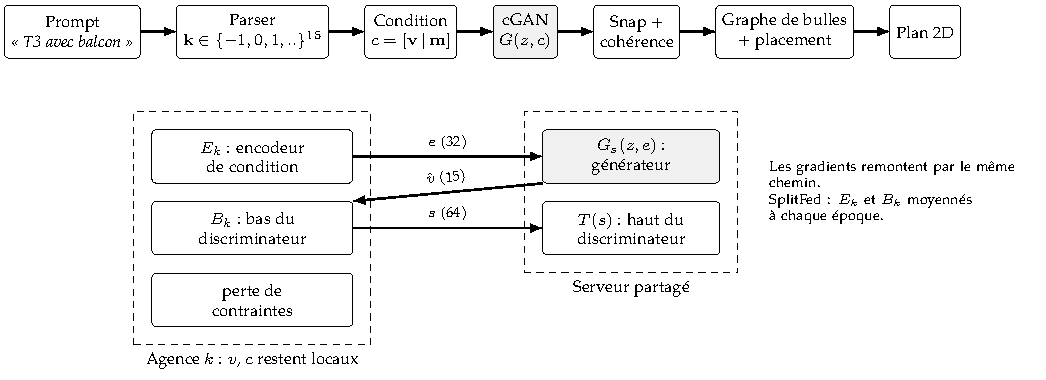
\includegraphics[width=\textwidth]{figures/architecture.pdf}
\caption{En haut, le pipeline d'inférence. En bas, le découpage du cGAN
pour le Split Learning en U : seuls les vecteurs $e$, $s$, le vecteur
généré $\hat v$ et leurs gradients franchissent la frontière ; les
programmes réels $v$ et les conditions $c$ restent chez l'agence.}
\label{fig:architecture}
\end{figure*}

\subsection{Représentation du programme et du graphe de bulles}

Nous appelons \emph{programme} un vecteur $v\in\mathbb{N}^{15}$. Ses neuf
premières composantes donnent le nombre de pièces de chaque type (salon,
chambre, douche, toilettes, couloir, bureau, cuisine, balcon, dressing),
et les six suivantes décrivent la topologie du graphe de bulles,
c'est-à-dire l'arbre de distribution du logement. Plutôt que de générer
une matrice d'adjacence de taille variable comme le fait
House-GAN~\cite{Nauata2020HouseGAN}, nous sommes partis du constat que,
dans un logement, la liberté de cet arbre porte essentiellement sur le
rattachement des pièces annexes. Six entiers suffisent donc à le
décrire : le nombre de salles d'eau privatives (suites), de WC intégrés à
la salle d'eau, de dressings attenants à une chambre, de balcons
desservis par une chambre, de cuisines desservies par le couloir
(cuisine fermée) et de bureaux ouverts sur le séjour. Cette
représentation reste compacte, se traduit toujours en un arbre valide
une fois ramenée dans le domaine réalisable (par exemple, pas plus de
suites que de chambres) et se prête directement à un perceptron
multicouche.

Chaque type de pièce dispose d'une plage de dimensions sur une grille
dont la cellule mesure 30\,cm (de 16 à 26\,m$^2$ pour le séjour, de 8 à
13\,m$^2$ pour une chambre) et d'une liste de voisins autorisés. Une
chambre peut ainsi s'ouvrir sur un couloir, une salle d'eau, un dressing
ou un balcon, et dans les petits logements le séjour joue le rôle de
dégagement. Nous avons également défini des liaisons interdites : WC ou
salle d'eau sur la cuisine, chambre sur chambre ou sur cuisine, WC sur
une chambre ou un bureau, et WC sur le séjour dès lors qu'un couloir
existe. Le générateur travaille uniquement sur $v$, la géométrie étant
confiée au placement (§\ref{sec:placement}). Ce choix découle
directement de l'expérience du prototype v1 : il rend la perte de
contraintes différentiable et confie les garanties fonctionnelles à un
algorithme que l'on peut vérifier, plutôt qu'au réseau.

\subsection{De la requête à la condition}

Le parser associe à chaque type de pièce une liste de synonymes
(« séjour », « sdb », « wc », « terrasse », etc.). Il reconnaît les
typologies (studio, T1 à T6), les nombres écrits en chiffres ou en
lettres, les négations comme « sans balcon », ainsi qu'une surface ou
une emprise (« T3 de 65\,m$^2$ », « plan 9$\times$11\,m »). Certaines
expressions fixent en outre la topologie : « suite parentale »,
« cuisine fermée » ou « ouverte », « WC séparés », « WC dans la salle de
bain », « chambre avec dressing » ou « coin bureau ». Lorsqu'une telle
expression suppose des pièces non mentionnées, celles-ci sont ajoutées ;
une suite parentale implique par exemple deux salles d'eau. Le parser
produit ainsi un vecteur $\mathbf{k}\in\{-1,0,1,\dots\}^{15}$, où $-1$
indique une valeur libre. La condition transmise au cGAN sépare la
valeur du masque :
\begin{equation}
  c = [\,\mathbf{v}\,|\,\mathbf{m}\,],\quad
  m_i = \mathbf{1}[k_i \ge 0],\quad
  v_i = m_i \min\!\big(1, k_i / M_i\big),
\end{equation}
où $M_i$ désigne le maximum observé pour la composante $i$ dans les
données. Sans ce masque, le réseau ne pourrait pas distinguer une
demande « sans balcon » d'une requête qui ne mentionne pas le balcon.

\subsection{GAN conditionnel}

Le générateur $G(z,c)$ et le discriminateur $D(v,c)$ sont des
perceptrons multicouches comptant respectivement \resParamsG{} et
\resParamsD{} paramètres, avec $z\in\mathbb{R}^{32}$. Pendant
l'entraînement, chaque programme réel est associé à une condition
obtenue en masquant aléatoirement entre 30 et 90\,\% de ses composantes,
ce qui apprend au modèle à compléter des requêtes plus ou moins
détaillées. Le générateur minimise
\begin{equation}
  \mathcal{L}_G = \mathcal{L}_{\text{adv}}
     + \lambda\,\frac{\sum_i m_i\,(G(z,c)_i - v_i)^2}{\sum_i m_i},
  \label{eq:loss}
\end{equation}
où le second terme pénalise l'écart aux valeurs imposées. Nous avons
retenu $\lambda=15$, valeur dont l'influence est étudiée plus loin. Le
discriminateur est entraîné avec une entropie croisée et un lissage des
étiquettes (0,9 et 0,1).

\subsection{Rétablissement des contraintes}

À l'inférence, la sortie du générateur est dénormalisée et arrondie,
puis les valeurs imposées par la requête sont rétablies telles quelles
(étape que nous appelons \emph{snap}). Trois règles minimales
s'appliquent ensuite : un salon et une cuisine sont toujours présents,
et un couloir est ajouté à partir de deux chambres. Le snap assure le
respect des demandes explicites, y compris lorsqu'elles sortent de la
distribution apprise (cinq chambres, alors que les données n'en
comptent pas plus de quatre), tandis que le cGAN reste responsable de
tout ce que la requête ne précise pas.

\subsection{Placement guidé par le graphe de bulles}
\label{sec:placement}

La version précédente du placement (v2), héritée du mémoire, accolait
chaque pièce à un voisin autorisé choisi au hasard, puis ouvrait une
porte sur chaque contact autorisé. Sur 300 programmes, nous avons
constaté qu'elle produisait en moyenne 1,9 porte par chambre et 1,6 par
salle d'eau, transformant ces pièces en pièces de passage. Elle laissait
aussi 17\,\% des chambres sans accès direct à une circulation, faisait
ouvrir 10\,\% des WC sur le séjour ou la cuisine, et donnait une emprise
très découpée (compacité de 0,66). Le placement v3 que nous proposons se
déroule en quatre étapes.

\paragraph{Construction du graphe.}
Le programme et sa topologie permettent d'abord de construire l'arbre
de distribution du logement, dont le séjour est la racine. Le couloir,
lorsqu'il existe, y est rattaché et dessert les chambres, la salle d'eau
commune, les WC et le bureau ; en son absence, ce rôle revient au
séjour. Les six variables de topologie déterminent ensuite les autres
rattachements : une salle d'eau supplémentaire peut être placée sur la
circulation ou en suite, les WC sur le couloir ou dans la salle d'eau
commune, le dressing et le balcon sur une chambre ou sur une
circulation, la cuisine sur le séjour ou sur le couloir, et le bureau
sur le couloir ou sur le séjour. Une salle d'eau commune est toujours
conservée. Lorsque aucune topologie n'est fournie, des règles fixes
s'appliquent ; elles nous servent de référence dans l'ablation.

\paragraph{Placement des pièces.}
Les pièces sont posées dans l'ordre de l'arbre, chacune contre sa pièce
parente. Leur taille est tirée dans leur plage, puis mise à l'échelle
lorsque la requête précise une surface, selon le facteur
$s=\sqrt{S_{\text{demandée}}/S_{\text{attendue}}}$ borné à
$[0{,}75 ; 1{,}5]$. La longueur du couloir dépend du nombre de pièces
qu'il dessert. Parmi les positions qui touchent la pièce parente sur au
moins 90\,cm sans chevauchement, nous retenons la plus proche du centre
des pièces déjà placées. Si la pièce parente n'a plus de place, les
autres pièces autorisées sont essayées, puis les autres pièces non
interdites.

\paragraph{Portes.}
Les portes forment un arbre couvrant de coût minimal sur le graphe des
contacts entre pièces. Le coût d'un contact vaut 0 s'il correspond à une
arête du graphe de bulles, 1 s'il s'agit d'un contact autorisé avec une
circulation, 2 pour un autre contact autorisé, 10 pour un contact neutre
et 100 pour un contact interdit. Seule la zone jour (séjour, cuisine,
balcon, couloir) peut recevoir des portes supplémentaires formant une
boucle, à moins que cela ne contredise le graphe ; une cuisine fermée ne
s'ouvre donc pas sur le séjour. Enfin, une porte d'entrée est percée dans
le plus long mur extérieur du couloir, ou à défaut du séjour.

\paragraph{Essais multiples.}
Le placement étant aléatoire, jusqu'à cinq essais sont réalisés. Nous
retenons le premier plan complet, connexe, sans porte interdite et dont
toutes les pièces sont accessibles depuis l'entrée sans traverser de
pièce privée, ou, à défaut, le meilleur plan selon ces critères. Il faut
donc garder à l'esprit que la connexité et l'absence de portes
interdites relèvent de l'algorithme de placement, et non des
performances du GAN.

\subsection{Split Learning en U}

Pour l'entraînement collaboratif, le cGAN est découpé en quatre modules
(Fig.~\ref{fig:architecture}). Chaque agence $k$ dispose d'un encodeur
de condition $E_k : c\mapsto e\in\mathbb{R}^{32}$ et de la partie basse
du discriminateur $B_k : (v,c)\mapsto s\in\mathbb{R}^{64}$, tandis que le
serveur héberge le générateur $G_s(z,e)$ et la partie haute du
discriminateur $T(s)$. Un pas d'entraînement comporte deux phases.
Dans la phase du discriminateur, l'agence envoie $e=E_k(c)$ et reçoit
en retour $\hat v = G_s(z,e)$ ; elle calcule ensuite
$s_{\text{réel}}=B_k(v,c)$ et $s_{\text{faux}}=B_k(\hat v,c)$, qu'elle
transmet au serveur. Celui-ci calcule la perte, met à jour $T$ et
renvoie les gradients de $s$, grâce auxquels l'agence met à jour $B_k$.
La phase du générateur suit le même aller-retour : la perte
adversariale est calculée sur le serveur et la perte de contraintes
chez l'agence, qui est la seule à connaître $c$, puis les gradients
redescendent par $\hat v$ vers $G_s$ et par $e$ vers $E_k$. Les
programmes $v$ et les conditions $c$ ne quittent donc jamais l'agence.

Nous comparons trois variantes. Dans la variante \textbf{SL}, chaque
agence conserve ses propres modules $E_k$ et $B_k$, et les agences sont
servies à tour de rôle. Dans la variante \textbf{SplitFed}, ces modules
sont moyennés (FedAvg) à la fin de chaque époque. La variante
\textbf{SplitFed+bruit} ajoute en outre un bruit gaussien
($\sigma=0{,}5$) à $e$ et $s$ avant leur envoi. Dans notre
implémentation, la frontière entre agence et serveur est matérialisée
par un détachement explicite des tenseurs et un renvoi manuel des
gradients, ce qui permet de mesurer exactement les volumes échangés ;
les échanges ont toutefois lieu au sein d'un même processus.

\subsection{Données}

En l'absence de corpus public de programmes annotés en français, nous
avons généré les programmes. Une typologie est d'abord tirée (T1 10\,\%,
T2 20\,\%, T3 35\,\%, T4 25\,\%, T5 10\,\%), puis les pièces annexes selon
des probabilités simples (balcon 50\,\%, bureau 30\,\%, etc.), et enfin
la topologie. Celle-ci suit des préférences qui dépendent du programme :
une salle d'eau supplémentaire devient une suite dans 85\,\% des cas, les
WC sont intégrés à la salle d'eau dans 70\,\% des logements sans couloir
contre 15\,\% des autres, un dressing est attenant à une chambre dans
80\,\% des cas et une cuisine est fermée dans 35\,\% des cas lorsqu'il y a
un couloir. C'est précisément cette dépendance que le cGAN doit
apprendre. Un programme n'est conservé que si le placement parvient à le
réaliser entièrement en trois essais au plus, avec un plan connexe et au
moins 90\,\% de portes conformes. Le placement v3 réalise ainsi
\resDsAcceptance{} des programmes tirés, les échecs provenant surtout de
rattachements impossibles faute de place autour de la pièce parente. Le
jeu final compte \resDsN{} programmes, dont \resDsUnique{} distincts
(\resDsUniquePieces{} si l'on ignore la topologie), avec
\resDsMeanRooms{} pièces en moyenne. Il est réparti à raison de 90\,\%
pour l'apprentissage et 10\,\% pour le test. Nous dirons qu'un programme
généré est \emph{plausible} lorsqu'il appartient à l'ensemble des
programmes réalisables observés.


% ============================================================
\section{Protocole expérimental}
% ============================================================

\paragraph{Métriques.}
Le \emph{respect brut} mesure la part des valeurs imposées que la sortie
arrondie du cGAN reproduit exactement, avant le snap. Le \emph{respect
dans le plan} applique la même mesure au plan final, en comptant les
pièces effectivement placées et en relisant la topologie sur les
portes ; le \emph{respect du graphe} la restreint aux variables de
topologie, pour les requêtes qui en imposent. La \emph{plausibilité} a
été définie plus haut. La \emph{diversité} correspond au nombre de
programmes distincts obtenus pour une même requête, et la
\emph{diversité du graphe} au nombre de topologies distinctes. La
\emph{connectivité} est la part des pièces atteignables depuis le salon
en passant par les portes (parcours en largeur). Les \emph{portes
légales} désignent la part des portes reliant deux pièces dont
l'adjacence est autorisée, et l'\emph{adjacence} la part des pièces
ayant au moins un voisin autorisé accessible par une porte. Nous
mesurons également la part des plans \emph{sans porte interdite},
l'\emph{accès direct}, c'est-à-dire la part des pièces atteignables
depuis l'entrée sans traverser de pièce privée (chambre, salle d'eau,
WC, bureau ou dressing), une annexe pouvant toutefois être desservie par
sa pièce principale, ainsi que le nombre moyen de \emph{portes par pièce
privée}. La \emph{compacité} rapporte la surface des pièces à celle de
la boîte englobante, et l'\emph{écart de surface} mesure l'écart relatif
à la surface demandée lorsque la requête en précise une. Le
\emph{temps} couvre le parsing, la génération et le placement, sans le
rendu graphique.

\paragraph{Méthodes de référence.}
Toutes les méthodes utilisent le même parser, le même placement et le
même rendu ; seule change la façon de compléter les éléments libres.
Nous comparons la méthode proposée (\emph{cGAN+snap}) au cGAN sans snap
(\emph{cGAN brut}), à un tirage \emph{aléatoire} uniforme des éléments
libres dans $[0, M_i]$, et à un \emph{prior empirique} qui tire un
programme du jeu d'apprentissage compatible avec les contraintes, ou le
plus proche s'il n'en existe aucun.

\paragraph{Jeux d'évaluation.}
Au niveau du vecteur, 2\,000 conditions sont tirées du jeu de test en
masquant chaque composante avec une probabilité de 0,5. Au niveau du
plan, nous utilisons 22 requêtes qui couvrent les typologies, les pièces
annexes, les négations, trois surfaces imposées, cinq structures
imposées (« T4 avec suite parentale », « T3 avec cuisine fermée »,
« T2 avec WC séparés », etc.) et un cas hors distribution (« appart 5
chambres sans balcon »), chacune générée en 50 variantes.

\paragraph{Split Learning.}
Le jeu d'apprentissage est réparti entre trois agences selon le nombre
de chambres (A : 0 ou 1, B : 2, C : 3 ou 4). Pour rendre la répartition
moins tranchée, 70\,\% des programmes sont attribués à l'agence
correspondante et 30\,\% à une autre. Chaque configuration est entraînée
pendant \resSlEpochs{} époques et comparée au modèle centralisé au même
nombre d'époques. Les modèles sont évalués sur l'ensemble des conditions
de test, sur la partie correspondant aux typologies de chaque agence et
sur celle des autres agences.

\paragraph{Attaque par inversion.}
Nous supposons un serveur curieux qui connaît 20\,\% des couples
(programme, $s$) et entraîne un réseau à reconstruire $v$ à partir de
$s$. Nous mesurons la part des programmes exactement reconstruits sur
les 80\,\% restants, que nous comparons à une référence sans information
consistant à prédire le programme le plus fréquent.

\paragraph{Configuration.}
Les expériences ont été menées avec PyTorch sur Google Colab (GPU), avec
l'optimiseur Adam ($\text{lr}=2\times10^{-4}$, $\beta=(0{,}5;\,0{,}999)$),
des lots de 128 et une graine fixée à 42. L'entraînement centralisé dure
\resTrainMinutes{}\,min pour 200 époques.


% ============================================================
\section{Résultats}
% ============================================================

\subsection{Apprentissage du programme}

\begin{table}[tbp]
  \centering
  \caption{Évaluation au niveau du vecteur (conditions du jeu de test).
    « -- » : respect garanti par construction.}
  \label{tab:vectors}
  \setlength{\tabcolsep}{3.5pt}
  \begin{tabular}{lccc}
    \toprule
    Méthode & Respect brut & Plausibilité & Diversité \\
    \midrule
    Aléatoire     & -- & \resVecAleatoirePlausibilite & \resVecAleatoireDiversite \\
    Prior empir.  & -- & \resVecPriorPlausibilite & \resVecPriorDiversite \\
    cGAN brut     & \resVecCganBrutRespectBrut & \resVecCganBrutPlausibilite & -- \\
    cGAN + snap   & \resVecCganSnapRespectBrut & \resVecCganSnapPlausibilite & \resVecCganSnapDiversite \\
    \bottomrule
  \end{tabular}
\end{table}

Le Tableau~\ref{tab:vectors} permet d'isoler la contribution du réseau.
Sans snap, le cGAN reproduit \resVecCganBrutRespectBrut{} des valeurs
imposées et produit \resVecCganBrutPlausibilite{} de programmes
plausibles, alors qu'un tirage aléatoire des éléments libres n'en donne
que \resVecAleatoirePlausibilite{}. La plausibilité obtenue vient donc
bien de ce que le cGAN a appris de la distribution conditionnelle. Sa
diversité (\resVecCganSnapDiversite{} de programmes distincts pour une
même condition) est par ailleurs comparable à celle d'un tirage dans les
données (\resVecPriorDiversite{}). Le prior empirique reste, lui,
plausible par construction, et sur des données synthétiques une simple
recherche dans la base constitue une référence difficile à battre. Il
suppose cependant de disposer de toute la base en un même lieu, ce qui
n'est justement pas possible lorsque les données appartiennent à
plusieurs agences, alors que le cGAN peut être appris sans les
centraliser (§\ref{sec:sl-results}).

\subsection{Qualité des plans}

\begin{table*}[tbp]
  \centering
  \caption{Évaluation des plans complets : 22 requêtes $\times$ 50
    variantes, placement v3. Moyennes ; l'intervalle de
    confiance à 95\,\% est donné en points de pourcentage pour la méthode
    proposée.}
  \label{tab:plans}
  \begin{tabular}{lcccccc}
    \toprule
    Méthode & Respect (plan) & Plausibilité & Diversité & Connectivité
            & Portes légales & Adjacence \\
    \midrule
    Aléatoire     & \resPlanAleatoireRespectPlan & \resPlanAleatoirePlausibilite
                  & \resPlanAleatoireDiversite & \resPlanAleatoireConnectivite
                  & \resPlanAleatoirePortesLegales & \resPlanAleatoireAdjacence \\
    Prior empir.  & \resPlanPriorRespectPlan & \resPlanPriorPlausibilite
                  & \resPlanPriorDiversite & \resPlanPriorConnectivite
                  & \resPlanPriorPortesLegales & \resPlanPriorAdjacence \\
    cGAN brut     & \resPlanCganBrutRespectPlan & \resPlanCganBrutPlausibilite
                  & \resPlanCganBrutDiversite & \resPlanCganBrutConnectivite
                  & \resPlanCganBrutPortesLegales & \resPlanCganBrutAdjacence \\
    \textbf{cGAN + snap} & \resPlanCganSnapRespectPlan{} {\scriptsize$\pm$\resPlanCganSnapRespectPlanCi}
                  & \resPlanCganSnapPlausibilite{} {\scriptsize$\pm$\resPlanCganSnapPlausibiliteCi}
                  & \resPlanCganSnapDiversite{} {\scriptsize$\pm$\resPlanCganSnapDiversiteCi}
                  & \resPlanCganSnapConnectivite{} {\scriptsize$\pm$\resPlanCganSnapConnectiviteCi}
                  & \resPlanCganSnapPortesLegales{} {\scriptsize$\pm$\resPlanCganSnapPortesLegalesCi}
                  & \resPlanCganSnapAdjacence{} {\scriptsize$\pm$\resPlanCganSnapAdjacenceCi} \\
    \bottomrule
  \end{tabular}
\end{table*}

\begin{figure}[tbp]
  \centering
  \figorplaceholder{figures/fig_exemples_plans.png}{\linewidth}
  \caption{Plans générés par cGAN + snap pour quatre requêtes, dont un
    hors distribution (5 chambres). Murs porteurs en trait épais,
    portes avec arc de débattement, 1 cellule = 30\,cm.}
  \label{fig:exemples}
\end{figure}

Le Tableau~\ref{tab:plans} et la Fig.~\ref{fig:exemples} portent sur la
chaîne complète. La connectivité est très élevée pour toutes les
méthodes, mais elle découle du placement et ne peut pas être attribuée
au cGAN. Le snap fait passer le respect de la requête dans le plan de
\resPlanCganBrutRespectPlan{} à \resPlanCganSnapRespectPlan{}, avec en
contrepartie une plausibilité plus faible (\resPlanCganSnapPlausibilite{}
contre \resPlanCganBrutPlausibilite{}). Cet écart était attendu, puisque
le snap impose parfois des combinaisons absentes de la base ; c'est le
cas de la requête « appart 5 chambres sans balcon », dont la
plausibilité est nulle, le jeu de données s'arrêtant à quatre chambres.
Par rapport au tirage aléatoire (\resPlanAleatoirePlausibilite{}), le
cGAN multiplie la plausibilité par près de cinq, tout en restant en deçà
du prior empirique (\resPlanPriorPlausibilite{}), pour la raison
indiquée plus haut.

Notons qu'une première série d'expériences avait révélé une incohérence
dans nos règles. Un WC ne pouvait pas s'ouvrir sur le séjour, si bien que
le filtre de réalisabilité écartait tous les T2 sans couloir dont les WC
étaient séparés de la salle d'eau, et que la requête « T2 avec WC
séparés » obtenait une plausibilité nulle. Après correction, cette
liaison étant désormais autorisée en l'absence de couloir, la part de
programmes réalisables est passée de 88,8\,\% à \resDsAcceptance{} et la
plausibilité de cette requête à 0,84. Les résultats présentés ici sont
ceux du système corrigé.

\begin{table}[tbp]
  \centering
  \caption{Qualité architecturale selon le placement (mêmes programmes,
    générés par cGAN + snap).}
  \label{tab:placement}
  \setlength{\tabcolsep}{3pt}
  \begin{tabular}{lccc}
    \toprule
    & v2 & v3, 1 essai & \textbf{v3} \\
    \midrule
    Portes légales        & \resPlanCganSnapPlacementVDeuxPortesLegales
                          & \resPlanCganSnapUnEssaiPortesLegales & \resPlanCganSnapPortesLegales \\
    Sans porte interdite  & \resPlanCganSnapPlacementVDeuxSansPorteInterdite
                          & \resPlanCganSnapUnEssaiSansPorteInterdite & \resPlanCganSnapSansPorteInterdite \\
    Accès direct          & \resPlanCganSnapPlacementVDeuxAccesDirect
                          & \resPlanCganSnapUnEssaiAccesDirect & \resPlanCganSnapAccesDirect \\
    Portes / pièce privée & \resPlanCganSnapPlacementVDeuxPortesPiecePrivee
                          & \resPlanCganSnapUnEssaiPortesPiecePrivee & \resPlanCganSnapPortesPiecePrivee \\
    Compacité             & \resPlanCganSnapPlacementVDeuxCompacite
                          & \resPlanCganSnapUnEssaiCompacite & \resPlanCganSnapCompacite \\
    Porte d'entrée        & \resPlanCganSnapPlacementVDeuxEntree
                          & \resPlanCganSnapUnEssaiEntree & \resPlanCganSnapEntree \\
    Écart de surface      & \resPlanCganSnapPlacementVDeuxEcartSurface
                          & \resPlanCganSnapUnEssaiEcartSurface & \resPlanCganSnapEcartSurface \\
    Temps (ms)            & \resPlanCganSnapPlacementVDeuxTLayout
                          & \resPlanCganSnapUnEssaiTLayout & \resPlanCganSnapTLayout \\
    \bottomrule
  \end{tabular}
\end{table}

Le Tableau~\ref{tab:placement} permet d'évaluer l'effet du placement à
programmes identiques. Le placement v3 réduit le nombre moyen de portes
des pièces privées de \resPlanCganSnapPlacementVDeuxPortesPiecePrivee{} à
\resPlanCganSnapPortesPiecePrivee{}, l'excédent par rapport à une porte
correspondant aux suites et aux salles d'eau qui intègrent les WC. Il
améliore la compacité, qui passe de
\resPlanCganSnapPlacementVDeuxCompacite{} à \resPlanCganSnapCompacite{},
ajoute une porte d'entrée et ramène l'écart à la surface demandée de
\resPlanCganSnapPlacementVDeuxEcartSurface{} à
\resPlanCganSnapEcartSurface{}, tout en étant plus de dix fois plus
rapide. Les essais multiples éliminent quant à eux les derniers cas de
pièces traversées, l'accès direct passant de
\resPlanCganSnapUnEssaiAccesDirect{} avec un seul essai à
\resPlanCganSnapAccesDirect{} avec cinq.

\paragraph{Temps de génération.}
Un plan est produit en \resPlanCganSnapTTotal{}\,ms en moyenne (médiane
de \resPlanTimeMedian{}\,ms, minimum de \resPlanTimeMin{}\,ms et maximum
de \resPlanTimeMax{}\,ms), dont moins de 0,1\,ms pour le cGAN lorsque
l'inférence est faite par lots. Le rendu en PNG ajoute
\resPlanCganSnapTRender{}\,ms, de sorte que c'est lui, et non le réseau ni
le placement, qui domine le temps total. À titre de comparaison, le
prototype du mémoire annonçait 0,376\,s par plan, rendu compris.

\subsection{Prédiction du graphe de bulles}

\begin{table}[tbp]
  \centering
  \caption{Graphe prédit par le cGAN ou déduit par des règles fixes
    (mêmes pièces, placement v3). Le respect du graphe porte sur les cinq
    requêtes qui imposent une structure.}
  \label{tab:graphe}
  \setlength{\tabcolsep}{4pt}
  \begin{tabular}{lcc}
    \toprule
    & Règles fixes & \textbf{cGAN} \\
    \midrule
    Respect du graphe imposé & \resPlanCganSnapGrapheReglesRespectGraphe & \resPlanCganSnapRespectGraphe \\
    Respect du prompt (plan)  & \resPlanCganSnapGrapheReglesRespectPlan & \resPlanCganSnapRespectPlan \\
    Diversité du graphe       & \resPlanCganSnapGrapheReglesDiversiteGraphe & \resPlanCganSnapDiversiteGraphe \\
    Plausibilité              & \resPlanCganSnapGrapheReglesPlausibilite & \resPlanCganSnapPlausibilite \\
    Accès direct              & \resPlanCganSnapGrapheReglesAccesDirect & \resPlanCganSnapAccesDirect \\
    Portes / pièce privée     & \resPlanCganSnapGrapheReglesPortesPiecePrivee & \resPlanCganSnapPortesPiecePrivee \\
    \bottomrule
  \end{tabular}
\end{table}

\begin{figure*}[tbp]
  \centering
  \figorplaceholder{figures/apercu_topologies.png}{\textwidth}
  \caption{Un même programme (T3 avec deux salles d'eau, dressing,
    balcon et bureau) réalisé avec trois topologies : règles fixes ;
    suite parentale et cuisine fermée ; WC dans la salle d'eau, bureau
    ouvert sur le séjour et balcon desservi par une chambre. Sous chaque
    plan figure la topologie relue sur les portes.}
  \label{fig:topologies}
\end{figure*}

Le Tableau~\ref{tab:graphe} compare, à pièces égales, la topologie
prédite par le cGAN à celle que produisent des règles fixes. Ces règles
ne peuvent satisfaire une demande de structure que si elle correspond à
leur choix par défaut, alors que le graphe prédit, une fois les
contraintes rétablies, la satisfait dès lors que le placement parvient à
le réaliser (Fig.~\ref{fig:topologies}). Sur les cinq requêtes
structurelles, le graphe demandé est obtenu dans
\resPlanCganSnapRespectGraphe{} des cas avec la prédiction, contre
\resPlanCganSnapGrapheReglesRespectGraphe{} avec les règles fixes. Ces
dernières échouent par exemple systématiquement sur « T3 avec cuisine
fermée », et dans 92\,\% des cas sur « T2 avec WC séparés ». La
prédiction fait en outre plus que doubler la diversité des graphes
obtenus pour une même requête (\resPlanCganSnapDiversiteGraphe{} contre
\resPlanCganSnapGrapheReglesDiversiteGraphe{}), au prix d'un léger recul
de la plausibilité (\resPlanCganSnapPlausibilite{} contre
\resPlanCganSnapGrapheReglesPlausibilite{}) qui s'explique par un espace
de programmes plus vaste. Les garanties apportées par le placement
restent inchangées. À titre de comparaison, le placement v2, qui ne
tient pas compte du graphe, n'en réalise que
\resPlanCganSnapPlacementVDeuxRespectGraphe{}.

\subsection{Influence du poids $\lambda$}

\begin{table}[tbp]
  \centering
  \caption{Effet de $\lambda$ (Éq.~\ref{eq:loss}), 60 époques.}
  \label{tab:ablation}
  \begin{tabular}{lccc}
    \toprule
    $\lambda$ & Respect brut & Plausibilité & Diversité \\
    \midrule
    0  & \resAblLambdaZeroPZeroRespectBrut & \resAblLambdaZeroPZeroPlausibiliteSnap & \resAblLambdaZeroPZeroDiversite \\
    1  & \resAblLambdaUnPZeroRespectBrut & \resAblLambdaUnPZeroPlausibiliteSnap & \resAblLambdaUnPZeroDiversite \\
    5  & \resAblLambdaCinqPZeroRespectBrut & \resAblLambdaCinqPZeroPlausibiliteSnap & \resAblLambdaCinqPZeroDiversite \\
    15 & \resAblLambdaUnCinqPZeroRespectBrut & \resAblLambdaUnCinqPZeroPlausibiliteSnap & \resAblLambdaUnCinqPZeroDiversite \\
    50 & \resAblLambdaCinqZeroPZeroRespectBrut & \resAblLambdaCinqZeroPZeroPlausibiliteSnap & \resAblLambdaCinqZeroPZeroDiversite \\
    \bottomrule
  \end{tabular}
\end{table}

Le conditionnement suffit à lui seul ($\lambda=0$) à reproduire
\resAblLambdaZeroPZeroRespectBrut{} des valeurs imposées. La perte de
contraintes comble l'essentiel de l'écart restant, puisque le respect
dépasse 99\,\% dès $\lambda=5$. Elle ne dégrade pas la plausibilité
(\resAblLambdaZeroPZeroPlausibiliteSnap{} pour $\lambda=0$ et
\resAblLambdaUnCinqPZeroPlausibiliteSnap{} pour $\lambda=15$), mais
s'accompagne d'une légère baisse de la diversité, qui passe de
\resAblLambdaZeroPZeroDiversite{} à \resAblLambdaCinqZeroPZeroDiversite{}
pour $\lambda=50$, le générateur devenant un peu plus prudent. La valeur
retenue, $\lambda=15$, se situe sur le palier où le respect est
maximal.

\subsection{Entraînement en Split Learning}
\label{sec:sl-results}

\begin{table*}[tbp]
  \centering
  \caption{Entraînement collaboratif sur trois agences non-IID
    (\resSlEpochs{} époques). Respect brut des contraintes / plausibilité,
    sur l'ensemble des conditions de test, sur le segment propre de
    chaque agence et sur les segments des autres agences.}
  \label{tab:split}
  \begin{tabular}{lcccccc}
    \toprule
    & \multicolumn{2}{c}{Global} & \multicolumn{2}{c}{Segment propre}
    & \multicolumn{2}{c}{Segments étrangers} \\
    \cmidrule(lr){2-3}\cmidrule(lr){4-5}\cmidrule(lr){6-7}
    Configuration & Respect & Plaus. & Respect & Plaus. & Respect & Plaus. \\
    \midrule
    Centralisé (référence, non confidentiel)
      & \resSlCentraliseGlobalRespectBrut & \resSlCentraliseGlobalPlausibilite
      & \resSlCentralisePropreRespectBrut & \resSlCentraliseProprePlausibilite
      & \resSlCentraliseEtrangerRespectBrut & \resSlCentraliseEtrangerPlausibilite \\
    Local seul (sans collaboration)
      & \resSlLocalGlobalRespectBrut & \resSlLocalGlobalPlausibilite
      & \resSlLocalPropreRespectBrut & \resSlLocalProprePlausibilite
      & \resSlLocalEtrangerRespectBrut & \resSlLocalEtrangerPlausibilite \\
    SL (modules client privés)
      & \resSlSlGlobalRespectBrut & \resSlSlGlobalPlausibilite
      & \resSlSlPropreRespectBrut & \resSlSlProprePlausibilite
      & \resSlSlEtrangerRespectBrut & \resSlSlEtrangerPlausibilite \\
    SplitFed
      & \resSlSplitfedGlobalRespectBrut & \resSlSplitfedGlobalPlausibilite
      & \resSlSplitfedPropreRespectBrut & \resSlSplitfedProprePlausibilite
      & \resSlSplitfedEtrangerRespectBrut & \resSlSplitfedEtrangerPlausibilite \\
    SplitFed + bruit ($\sigma=0{,}5$)
      & \resSlSplitfedBruitGlobalRespectBrut & \resSlSplitfedBruitGlobalPlausibilite
      & \resSlSplitfedBruitPropreRespectBrut & \resSlSplitfedBruitProprePlausibilite
      & \resSlSplitfedBruitEtrangerRespectBrut & \resSlSplitfedBruitEtrangerPlausibilite \\
    \bottomrule
  \end{tabular}
\end{table*}

\begin{figure}[tbp]
  \centering
  \figorplaceholder{figures/fig_split_training.png}{\linewidth}
  \caption{Convergence des variantes de Split Learning comparée à
    l'entraînement centralisé.}
  \label{fig:split}
\end{figure}

Le Tableau~\ref{tab:split} répond à deux questions. Il s'agit d'abord de
savoir si la collaboration apporte quelque chose à une agence par
rapport à un entraînement local, en particulier sur les typologies
qu'elle connaît peu, puis de mesurer l'écart qui subsiste avec un modèle
centralisé, lequel suppose de partager les données.

Une agence qui travaille seule obtient un modèle satisfaisant sur ses
propres typologies, mais moins fiable sur les autres, avec un respect
des contraintes qui descend à \resSlLocalEtrangerRespectBrut{} sur ces
dernières. SplitFed corrige en grande partie ce défaut, avec
\resSlSplitfedEtrangerRespectBrut{} de respect et
\resSlSplitfedEtrangerPlausibilite{} de plausibilité sur les typologies
des autres agences, et atteint globalement
\resSlSplitfedGlobalRespectBrut{}, contre
\resSlCentraliseGlobalRespectBrut{} pour le modèle centralisé. L'écart
résiduel apparaît aussi sur les courbes de convergence
(Fig.~\ref{fig:split}), où la violation des contraintes reste environ
six fois plus élevée qu'en centralisé après 100 époques. La
plausibilité est en revanche du même ordre, voire légèrement supérieure,
ce qui laisse penser que le générateur est un peu plus conservateur. La
variante SL, dans laquelle chaque agence garde son propre encodeur de
condition, donne les moins bons résultats
(\resSlSlGlobalRespectBrut{} de respect et \resSlSlGlobalPlausibilite{}
de plausibilité), car le générateur partagé reçoit des représentations
de la condition qui diffèrent d'une agence à l'autre. Dans ce contexte
de données hétérogènes, la mise en commun des modules client opérée par
SplitFed s'avère donc indispensable.

\paragraph{Coût.}
Les modules situés chez les agences représentent \resSlClientShare{} des
paramètres (\resSlParamsClient{} contre \resSlParamsServer{} sur le
serveur). SplitFed échange \resSlSplitfedMoEpoch{}\,Mo d'activations et
de gradients par époque, soit \resSlSplitfedOctetsSample{} octets par
exemple, auxquels s'ajoutent \resSlSyncMoEpoch{}\,Mo de synchronisation.
Un FedAvg échangeant le modèle complet coûterait \resSlFlMoEpoch{}\,Mo
par époque, soit environ vingt-sept fois moins, et le jeu
d'apprentissage brut ne pèse lui-même qu'environ 1\,Mo. Avec un modèle
aussi petit et des données aussi compactes, le Split Learning ne se
justifie donc pas par un gain de bande passante. Son intérêt tient à
l'allègement du calcul chez les agences et, sous certaines conditions,
à la confidentialité. La situation serait différente avec des modèles
de grande taille~\cite{Singh2019CommEfficiency}.

\paragraph{Fuite d'information.}
Lorsque 20\,\% des couples sont connus, l'attaque par inversion
reconstruit exactement \resLeakSplitfedExact{} des programmes à partir
des activations de SplitFed, contre \resLeakSplitfedBaselineExact{} pour
la référence sans information, et seulement \resLeakSplitfedBruitExact{}
lorsque le bruit est activé. Sans protection, les activations échangées
protègent donc mal les programmes : l'attaquant en retrouve plus d'un
sur deux à l'identique et retrouve \resLeakSplitfedParEntree{} des
composantes, contre \resLeakSplitfedBaselineParEntree{} pour la
référence. Le bruit ramène l'attaque au niveau de cette référence
(\resLeakSplitfedBruitParEntree{} des composantes), ce qui signifie que
l'inverseur n'extrait plus d'information exploitable, pour un coût
modéré sur la qualité (respect global de
\resSlSplitfedBruitGlobalRespectBrut{} contre
\resSlSplitfedGlobalRespectBrut{}). Ces observations rejoignent les
attaques décrites dans la littérature~\cite{Pasquini2022,Gao2023PCAT} :
le Split Learning n'assure la confidentialité que s'il est accompagné
d'une protection explicite. Notons aussi que notre bruit gaussien
n'offre pas de garantie formelle, contrairement à la confidentialité
différentielle.


% ============================================================
\section{Discussion}
% ============================================================

\paragraph{Répartition des rôles entre le réseau et l'algorithme.}
Notre approche confie au cGAN ce qui relève d'une distribution, par
exemple les pièces qui accompagnent habituellement un T3 avec bureau, et
à un algorithme ce qui relève de contraintes strictes, comme
l'accessibilité de toutes les pièces. Ce partage rend les garanties
vérifiables, mais il implique aussi que la qualité géométrique du plan
dépend entièrement du placement. Or, même en v3, l'emprise reste
irrégulière (compacité de l'ordre de 0,75), l'orientation et
l'éclairage naturel ne sont pas pris en compte, et le graphe se limite à
un arbre de distribution à six degrés de liberté. Cette représentation
est bien plus restreinte que les graphes quelconques de
House-GAN~\cite{Nauata2020HouseGAN}, mais elle garantit que tout graphe
généré est valide et réalisable, et elle peut être pilotée par une
requête en langage courant. Le placement peut néanmoins ne pas réussir
à réaliser un rattachement demandé lorsque la pièce parente n'a plus de
place, ce que mesure justement le respect du graphe.

\paragraph{Retour sur le prototype v1.}
Le prototype du mémoire affichait une connectivité de 1,00 et une
conformité d'adjacence de 0,92. Avec le recul, ces chiffres provenaient
pour l'essentiel de la fonction de placement, puisque le gradient des
pertes d'adjacence et SSIM ne pouvait pas la traverser pour atteindre le
générateur. La version actuelle rend ce point explicite et mesure à part
la contribution du réseau (Tableau~\ref{tab:vectors}).

\paragraph{Limites.}
Ce travail présente plusieurs limites. Les programmes d'entraînement
sont synthétiques, de sorte que le modèle apprend la distribution que
nous avons définie et non celle de plans réels ; l'étape suivante
consistera à extraire des programmes de corpus de plans réels, comme
RPLAN~\cite{Wu2019RPLAN}, ou de plans fournis par des agences
partenaires. Les règles d'adjacence, les liaisons interdites et les
plages de dimensions ont été fixées à la main à partir des usages
courants du logement, sans s'appuyer sur une norme. Le Split Learning
est simulé au sein d'un seul processus, si bien que la latence du réseau
et le chiffrement des échanges (TLS) ne sont pas mesurés. L'attaque
étudiée reste simple, et des attaques plus fortes comme
PCAT~\cite{Gao2023PCAT} ou des défenses dédiées comme
NoPeek~\cite{Vepakomma2020NoPeek} restent à évaluer. Enfin, la diversité
et la plausibilité ne remplacent pas l'avis d'architectes, qu'il
faudrait recueillir lors d'une évaluation qualitative.


% ============================================================
\section{Conclusion}
% ============================================================

Nous avons présenté un générateur de plans 2D piloté par une requête
textuelle, qui associe un GAN conditionnel chargé de compléter le
programme à un placement procédural garantissant la validité
fonctionnelle du plan, et nous l'avons entraîné en Split Learning en U
entre trois agences sans que leurs programmes ne quittent leurs locaux.
Les plans obtenus respectent \resPlanCganSnapRespectPlan{} des
contraintes de la requête, ne comportent aucune porte interdite et sont
produits en quelques millisecondes. La prédiction du graphe de bulles
porte le respect des structures demandées à
\resPlanCganSnapRespectGraphe{}. Entraîné en SplitFed, le modèle s'approche
du modèle centralisé (\resSlSplitfedGlobalRespectBrut{} contre
\resSlCentraliseGlobalRespectBrut{}) et dépasse les modèles locaux, à
condition toutefois de bruiter les activations échangées, faute de quoi
plus de la moitié des programmes peuvent être reconstruits.

Plusieurs prolongements sont envisagés : l'apprentissage sur des
programmes issus de plans réels, l'extension du conditionnement à
l'emprise et à l'orientation, la mise en place de protections offrant
des garanties formelles (confidentialité différentielle,
NoPeek~\cite{Vepakomma2020NoPeek}), un déploiement du protocole sur un
véritable réseau et l'export des plans vers les logiciels de CAO aux
formats DXF ou IFC.


% ============================================================
\section*{Disponibilité du code}

Le code source, le notebook \texttt{ArchiGAN\_SL\_v2.ipynb} et les poids
du modèle entraîné sont disponibles à l'adresse
\url{https://github.com/Kenny-19/Archi_GAN}. Le notebook permet de
reproduire l'ensemble des expériences ainsi que les tableaux et figures
de cet article (graine fixée à 42). Une démonstration en ligne, qui
exécute le générateur directement dans le navigateur, est accessible à
l'adresse \url{https://archigansite.vercel.app}.

\section*{Remerciements}

L'auteur remercie le Professeur Antoine Bagula (directeur) et
l'Ass. Benjamin Oleko (encadreur) pour leurs orientations scientifiques,
ainsi que l'Université Nouveaux Horizons.

\section*{Conflits d'intérêt}

L'auteur déclare n'avoir aucun conflit d'intérêt.

\bibliographystyle{unsrt}
\bibliography{references}

\end{document}
